\chapter{Aprendizaje Automático y \textit{AutoML}}\label{chap:1}

En este primer capítulo se aborda el marco teórico de la tesis, el cual se enfoca en diferentes temas clave dentro del campo de la inteligencia artificial y la minería de datos. En particular, se discute el aprendizaje automático, el descubrimiento de conocimiento en bases de datos, la minería de datos y la clasificación. Además, se introduce el concepto de AutoML, como herramienta para automatizar el proceso de preprocesado y optimización de hiperparámetros en la implementación de técnicas de aprendizaje automático. Por último, se destaca la importancia de la plataforma KNIME como una herramienta útil para la implementación de técnicas de AutoML y análisis de datos.

\section{Aprendizaje Automático}
Uno de los campos más destacados dentro de la IA es el Machine Learning (aprendizaje automático), que es un enfoque que utiliza algoritmos y modelos matemáticos para permitir que los sistemas aprendan de los datos y realicen tareas específicas sin ser programados explícitamente.
Se define el Aprendizaje Automático como un conjunto de métodos que pueden detectar automáticamente patrones en los datos y luego usar los patrones descubiertos para predecir datos futuros o para realizar otros tipos de toma de decisiones bajo incertidumbre \citep{murphy2012machine}. Es decir, es el proceso en el que las computadoras descubren cómo hacer cosas sin estar específicamente programadas para hacerlo \citep{Praba2021}.
Por lo tanto, el objetivo principal del aprendizaje automático es estudiar, diseñar y mejorar modelos matemáticos que se pueden entrenar (una vez o continuamente) con datos relacionados con el contexto (proporcionados por un entorno genérico), para inferir el futuro y tomar decisiones sin completo. conocimiento de todos los elementos que influyen (factores externos) \citep{bonaccorso2017machine}. \\
Existen varios tipos de aprendizaje en Machine Learning, cada uno con sus propias técnicas y enfoques. A continuación, se presenta una breve descripción de algunos de los tipos de aprendizaje más comunes:
\begin{itemize}
	\item Aprendizaje supervisado: se refiere a cualquier proceso de aprendizaje automático que aprende una función de un tipo de entrada a un tipo de salida utilizando datos que comprenden ejemplos que tienen valores de entrada y salida. Dos ejemplos típicos de aprendizaje supervisado son el aprendizaje de clasificación y la regresión \citep{sammut2011encyclopedia}. 
	\item Aprendizaje no supervisado: se refiere a cualquier proceso de aprendizaje automático que busca aprender la estructura en ausencia de un resultado identificado o retroalimentación. Tres ejemplos típicos de aprendizaje no supervisado son agrupamiento, reglas de asociación y mapas de autoorganización \citep{sammut2011encyclopedia}. 
	\item Aprendizaje por refuerzo: describe una gran clase de problemas de aprendizaje característicos de los agentes autónomos que interactúan en un entorno: problemas de toma de decisiones secuenciales con recompensa retrasada. Los algoritmos de aprendizaje por refuerzo buscan aprender una política (mapeo de estados a acciones) que maximice la recompensa recibida a lo largo del tiempo \citep{sammut2011encyclopedia}. 
	\item Aprendizaje semisupervisado: es una clase de técnicas de aprendizaje automático que hacen uso de ejemplos etiquetados y no etiquetados al aprender un modelo. En un enfoque, los ejemplos etiquetados se usan para aprender modelos de clase y los ejemplos no etiquetados se usan para refinar los límites entre clases \citep{Han2011}.
\end{itemize}
En resumen, Machine Learning es una técnica que permite a las computadoras aprender patrones a partir de datos, con el objetivo de realizar predicciones o clasificaciones precisas en datos nuevos. Sin embargo, antes de aplicar técnicas de Machine Learning a un conjunto de datos, es necesario realizar una serie de procesos previos, como la selección y preprocesamiento de datos, la selección de técnicas de aprendizaje adecuadas, la evaluación y ajuste de modelos, entre otros. De esta manera, el proceso de  descubrimiento de conocimiento en bases de datos complementa al Machine Learning, permitiendo una exploración más completa de los datos y una selección más adecuada de las técnicas de aprendizaje.

\section{Proceso de descubrimiento de conocimiento en bases de datos}\label{kdd}
La Extracción de Conocimiento en Bases de Datos (\textit{Knwodlege Discovery from Databases}, o \textit{KDD} por sus siglas en inglés) se define como: “el proceso no trivial de identificar patrones válidos, novedosos, potencialmente útiles y, en última instancia, comprensibles a partir de los datos” \citep{orallo2004}. Este proceso está compuesto por una serie de etapas o fases, descritas a continuación:
\begin{itemize}
	\item Integración y recopilación: Se requiere poseer todos los datos que sean de utilidad a partir de las necesidades de la organización. Determina las fuentes de información que pueden ser útiles y dónde conseguirlas. Como parte del desarrollo de esta fase es necesario diseñar o conocer el modo en que se van a organizar e integrar los datos; con el fin de eliminar redundancias e inconsistencias.
	\item Selección, limpieza y transformación: Se seleccionan los datos más relevantes y que aporten mejor información, garantizando que el dato tenga la mejor calidad posible logrando obtener las vistas minables, con los datos listos para la aplicación del algoritmo.
	\item Algoritmos de Minería de datos: A través de la vista minable obtenida en la fase anterior se aplican los algoritmos de extracción del conocimiento.
	\item Evaluación e Interpretación: El objetivo de esta etapa es medir la calidad de los modelos obtenidos utilizando diferentes métricas de calidad. Las cuales dependen de las técnicas de minería de datos que se utilicen. La interpretación de los resultados se apoya en el uso de técnicas de visualización y de representación con el fin de entender mejor el conocimiento aportado. 
	\item Difusión y uso: En esta etapa, se integra el conocimiento obtenido de la comprensión del negocio, con el conocimiento de los modelos de minería de datos usado en la toma de decisiones de los especialistas. La monitorización de los patrones debe realizarse, pues en ocasiones resulta necesaria la reevaluación del modelo, su reentrenamiento o incluso su reconstrucción total.
\end{itemize}
Tras el aumento de  grandes volúmenes de información en toda institución donde se almacenen datos históricos, ahora informatizados en bases de datos digitales, es necesaria la extracción de información valiosa a través de patrones ocultos en estos datos. Sin embargo, esta cantidad de información sobrepasa las capacidades de los analistas de estas instituciones, provocando la necesidad del empleo de técnicas automatizadas. De aquí, surge como una nueva necesidad la minería de datos, siendo parte del proceso KDD.		

\section{Minería de Datos}
Según \citep{orallo2004}, la minería de datos es definida como el proceso de extraer conocimiento útil y comprensible, previamente desconocido, desde grandes cantidades de datos almacenados en distintos formatos. \\
El conocimiento extraído se puede presentar en forma de relaciones, patrones o reglas inferidos de los datos, o en forma de descripción un poco más concisa. Estos constituyen un modelo de datos analizados. Estos modelos, o tareas, se categorizan en predictivas y descriptivas \citep{orallo2004}. \\
En las tareas predictivas, los ejemplos están etiquetados y se emplean para estimar valores futuros o desconocidos de variables de interés. En este entorno se encuentra el aprendizaje supervisado. En cambio, las tareas descriptivas son empleadas en el descubrimiento de propiedades de los datos examinados donde los ejemplos no se encuentran etiquetados. Aquí se pone de manifiesto el aprendizaje no supervisado. En \citep{orallo2004} se describen las tareas de minería de datos como sigue:
\begin{itemize}
	\item Clasificación: La clasificación se encarga de examinar las características de un registro u objeto, y de esta forma asignarle una clase predefinida. Estas clases son valores discretos. Para ello, se tiene que construir un modelo a partir de datos previamente clasificados. Como variantes a la clasificación, existe el aprendizaje de “rankings”, aprendizaje de preferencias y el aprendizaje de probabilidad, entre otros. 
	\item Regresión: A diferencia de la clasificación, el valor a predecir es numérico. Consiste en aprender una función real que calcula un valor para un atributo real. Su objetivo es minimizar el error entre el valor predicho y el valor real.
	\item  Correlaciones: Son empleadas para examinar el grado de similitud de los valores de dos variables numéricas. Se basa en el cálculo de correlación de variables numéricas usando la estadística. Este método trata de determinar si el comportamiento de dos variables numéricas está relacionado.
	\item Reglas de asociación: Las reglas de asociación son situaciones o características que ocurren en un mismo instante de tiempo. Pueden ser relaciones causales o casuales. Representan patrones de comportamiento entre los datos en función de la aparición conjunta de valores de dos o más atributos. Las medidas habituales propuestas en \citep{Agrawal1519}	para establecer la idoneidad y el interés de una regla de asociación son la confianza y el soporte.
	\item	Agrupamiento (Clustering): Para realizar esta tarea se parte de datos sin clasificar, teniendo como objetivo segmentar un grupo de datos diversos en subgrupos. Los miembros de cada grupo (clúster, por su definición en inglés) deben tener mucho en común entre sí y, a su vez, diferenciarse del resto de elementos de otros grupos. Dado que la clasificación de estos grupos no se conoce previamente, es el minero el encargado de darles un significado.
\end{itemize}

\subsection{Clasificación}
En el uso común, la palabra clasificación significa colocar las cosas en categorías, agruparlas de alguna manera útil. Nosotros, como humanos, generalmente hacemos esto porque las cosas en un grupo, llamado \textit{clase} en aprendizaje automático, comparten características comunes \citep{sammut2011encyclopedia}. \\
En aprendizaje automático, la clasificación, se utiliza para identificar a qué clase o categoría pertenece una determinada observación o registro, basándose en un conjunto de características o variables. En esta, se utiliza un algoritmo para construir un modelo predictivo que asigne una etiqueta de clase a cada observación en función de sus características. Este modelo se entrena utilizando un conjunto de datos etiquetados previamente, y luego se aplica a nuevos datos para hacer predicciones \citep{sammut2011encyclopedia}.

\subsubsection{Clasificación con Árboles de Decisión}
La clasificación con árboles de decisión es un método popular en la minería de datos y en el aprendizaje automático supervisado, se utiliza para predecir la clase o categoría de un objeto o registro. Los Árboles de Decisión son unos de los modelos más populares, su representación es de fácil entendimiento, incluso por personas no afines al área, pues su construcción en sencilla: las hojas toman los valores objetivos, mientras los atributos y sus posibles valores conforman los nodos y ramas respectivamente \citep{sammut2011encyclopedia}. \\
Basados en árboles de decisión existen otros algoritmos de clasificación como: ID3, C4.5 y CART. Cada uno de ellos fue desarrollado como una versión mejorada del anterior, pero todos tienen una alta eficiencia y tiempos de ejecución reducidos, lo que los hace igualmente populares en la actualidad \citep{javed2022performance}. Se comparan y analizan en \citep{gupta2017analysis}, donde se arrojan sus principales características:
\begin{itemize}
	\item ID3 (Iterative Dichotomiser 3): Basa su funcionamiento en la entropía y la ganancia de información. El árbol se construye iterativamente de arriba hacia abajo, eligiendo en cada caso el atributo con mayor ganancia de información, hasta que la información ganada sea cero o se haya llegado a todas las hojas \citep{javed2022performance}, \citep{gupta2017analysis}. Maneja datos nominales y no tolera valores faltantes.
	\item C4.5 (Classification 4.5): Desarrollado con el objetivo de mejorar los defectos de ID3. Añade la poda, desestimando las ramas sin aportes, que reduce los errores al clasificar como resultado de un gran número de ramas en el modelo \citep{sammut2011encyclopedia}, \citep{javed2022performance}, \citep{gupta2017analysis}. Adicionalmente maneja valores faltantes y numéricos. 
	\item CART (Classification and Regression Trees): Genera un árbol binario siguiendo el mismo enfoque entrópico que ID3, pero empleando el coeficiente de Gini como criterio de selección \citep{javed2022performance}, \citep{gupta2017analysis}. Es capaz de manejar datos faltantes, al igual que datos numéricos y nominales.
\end{itemize}

\subsubsection{Clasificación con Redes Neuronales}
Las redes neuronales o redes neuronales artificiales, son algoritmos de aprendizaje basados en una vaga analogía de cómo funciona el cerebro humano. El aprendizaje se logra ajustando los pesos en las conexiones entre nodos, que son análogas a las sinapsis y las neuronas \citep{sammut2011encyclopedia}. \\
Las primeras redes neuronales conocidas como pre-alimentadas, como la de la figura \ref{fig:red-neuronal-prealimentada}, se caracterizan por tener una arquitectura en la que cada capa de neuronas está conectada completamente con la capa siguiente, pero no con la capa anterior. Esto significa que la información fluye de forma unidireccional, sin retroalimentación \citep{abiodun2018state}. 
\begin{figure}[H]
	\centering
	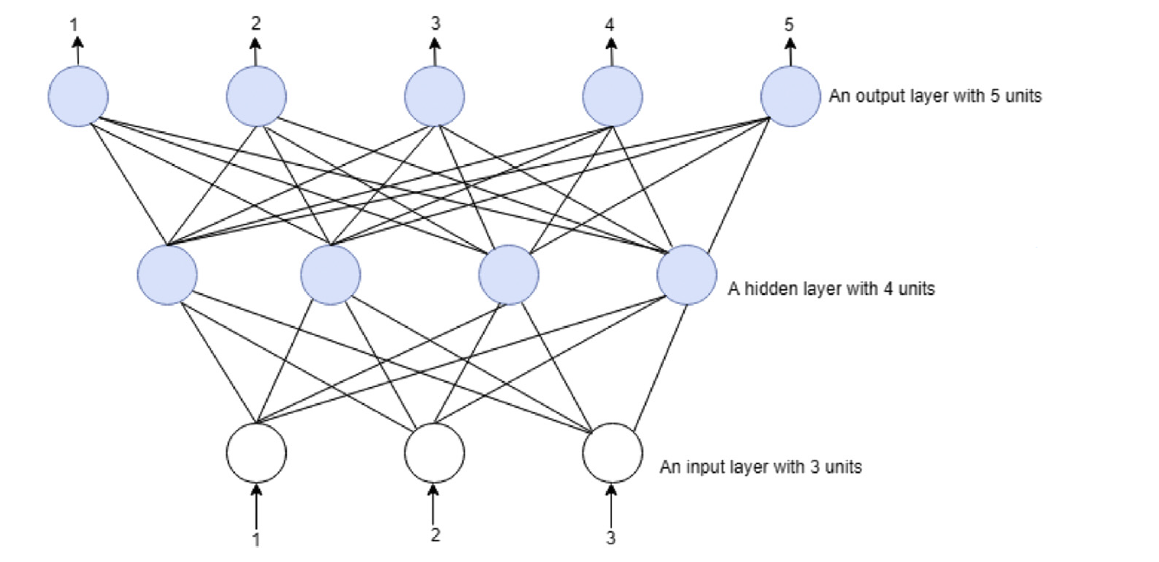
\includegraphics[width=0.7\linewidth]{figuras/capi 1/red-neuronal-prealimentada}
	\caption{Red Neuronal Pre-Alimentada \citep{abiodun2018state}}
	\label{fig:red-neuronal-prealimentada}
\end{figure}
Posteriormente, se desarrollaron las redes neuronales por retro propagación, como la presente en la figura \ref{fig:red-neuronal-retropropagacion}, que comparan la salida obtenida por la red con la salida deseada, y ajustan los pesos de las conexiones entre las neuronas de la red para reducir el error de predicción. La retro propagación se utiliza para calcular la contribución de cada peso en el error de la red, y así ajustarlos de manera adecuada \citep{abiodun2018state}.
\begin{figure}[H]
	\centering
	\includegraphics[width=0.6\linewidth]{figuras/capi 1/red-neuronal-retropropagación}
	\caption{Red neuronal por retro-propagación \citep{abiodun2018state}}
	\label{fig:red-neuronal-retropropagacion}
\end{figure}
Gracias a su gran versatilidad se pueden aplicar en una amplia variedad de campos y disciplinas para resolver problemas complejos de aprendizaje automático, como es el procesamiento del lenguaje natural, reconocimiento de voz e imágenes \citep{abiodun2018state}. Debido a la complejidad de sus modelos puede ser difícil su entendimiento, por lo que preferiblemente se utilizan en el contexto del reconocimiento de patrones, en la figura \ref{fig:red-neuronal-multicapa-compleja} se muestra un ejemplo de Red neuronal multicapa para el reconocimiento facial.
\begin{figure}[H]
	\centering
	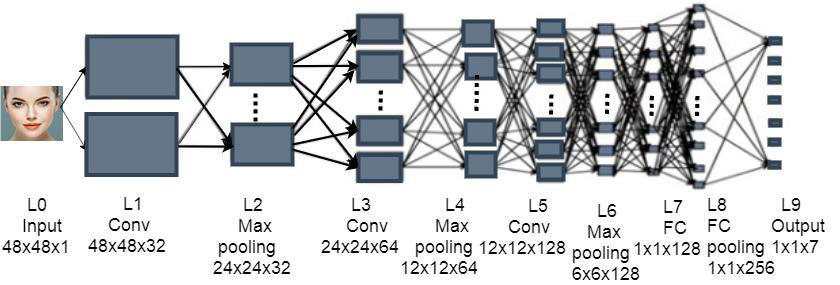
\includegraphics[width=0.7\linewidth]{figuras/capi 1/red-neuronal-multicapa-compleja}
	\caption{Red neuronal multicapa compleja \citep{abiodun2018state}}
	\label{fig:red-neuronal-multicapa-compleja}
\end{figure}

\subsubsection{Clasificación con Support Vector Machine}
Las Máquinas de Soporte Vectorial o Support Vector Machine (SVM) en inglés, son una clase de algoritmos lineales que se pueden usar para clasificación \citep{sammut2011encyclopedia}, cuyo objetivo es encontrar el hiperplano que mejor separa dos clases de datos en un espacio de alta dimensionalidad \citep{guenther2016support}. En la figura \ref{fig:ejemplos-de-posibles-hiperplanos-de-svm} se representa como el hiperplano H2 divide con mayor margen las clases que el hiperplano H1.
\begin{figure}[H]
	\centering
	\includegraphics[width=0.4\linewidth]{"figuras/capi 1/Ejemplos de posibles hiperplanos de SVM"}
	\caption{Ejemplos de posibles hiperplanos de SVM \citep{sammut2011encyclopedia}}
	\label{fig:ejemplos-de-posibles-hiperplanos-de-svm}
\end{figure}
Uno de los desafíos de SVM en problemas de clasificación de múltiples clases es cómo manejar la predicción de estas. En este contexto, existen dos enfoques principales:
\begin{itemize}
	\item Uno contra uno (One-vs-One): Durante la fase de predicción, cada clasificador binario vota por la clase que cree que es correcta y la clase con el mayor número de votos se selecciona como la clase final para el punto de datos dado. Este enfoque presenta la ventaja de que cada clasificador binario solo necesita ser entrenado en un subconjunto de los datos, lo que puede ser útil cuando hay grandes conjuntos de datos. Es más resistente a desequilibrios en la distribución de clases que otros enfoques de SVM \citep{guenther2016support}.
	\item Uno contra todos (One-vs-All): Entrena un clasificador binario para cada clase posible, donde el conjunto de datos de una clase se considera positivo y los datos de las otras clases se consideran negativos. Durante la fase de predicción, cada clasificador binario vota por su clase correspondiente y la clase con la mayor puntuación se selecciona como la clase final para el punto de datos dado. Fácil de implementar y puede funcionar bien en conjuntos de datos pequeños, pero puede ser menos preciso en conjuntos de datos grandes y complejos \citep{guenther2016support}.
\end{itemize}
Agregar que existen otros dos enfoques: Clasificación jerárquica (Hierarchical classification) y Clasificación por parejas (Pairwise classification). Cada uno de estos tiene sus propias ventajas y desventajas, y la elección de uno de ellos dependerá del tipo de datos y del problema que se esté tratando de resolver.

%Texto... Es una buena práctica culminar (o iniciar) cada epígrafe con una referencia al que sigue (o precede) para dar fluidez a su lectura y no se vea como un \emph{copia y pega} sin ninguna relación.
         
\section{\textit{AutoML}}

El campo del aprendizaje automático automatizado (AutoML) tiene como objetivo tomar decisiones de una manera automatizada, objetiva y basada en datos: el usuario simplemente proporciona datos y el sistema AutoML determina automáticamente el enfoque que funciona mejor para esta aplicación en particular \citep{hutter2019automated}. \\
AutoML (Automated Machine Learning) es una técnica que tiene como objetivo automatizar todo o parte del proceso de Machine Learning, incluyendo la selección de algoritmos, la optimización de hiperparámetros, la selección de características y la evaluación del rendimiento del modelo \citep{he2021automl}, \citep{tuggener2019automated}. La relación entre AutoML y Machine Learning es que AutoML es una técnica que se utiliza para automatizar el proceso de Machine Learning, lo que significa que se utiliza para automatizar todo o parte del proceso de selección del mejor modelo de Machine Learning para un conjunto de datos dado. La automatización del proceso de Machine Learning proporciona una solución eficiente y escalable para el análisis de grandes conjuntos de datos, lo que puede resultar en un ahorro significativo de tiempo y recursos para los profesionales de ciencia de datos y los investigadores. \\ 
Tras un análisis del estado del arte acerca del proceso de AutoML \citep{tuggener2019automated}, \citep{waring2020automated}, \citep{hutter2019automated}, \citep{he2021automl}, se pueden presentar las principales tareas como:
\begin{itemize}
	\item Selección de características: Esta tarea consiste en identificar las variables más relevantes para el problema de aprendizaje automático. 
	\item Pre-procesamiento de datos: La calidad de los datos de entrada es un factor crítico en el rendimiento de los modelos de aprendizaje automático. Las técnicas de preprocesamiento de datos se utilizan para limpiar, normalizar y transformar los datos de entrada en un formato que sea adecuado para el modelo. Existen varias técnicas efectivas de preprocesamiento de datos, incluyendo la eliminación de valores atípicos, la imputación de valores faltantes y la normalización y discretización de datos.
	\item Selección de modelo: identificar el modelo de aprendizaje automático que mejor se ajusta al problema dado.
	\item Ajuste de hiperparámetros: Los modelos de aprendizaje automático tienen varios parámetros que afectan su rendimiento, y encontrar los valores óptimos de estos parámetros es una tarea importante para mejorar el rendimiento del modelo. El estado del arte ha demostrado que existen varias técnicas para el ajuste de hiperparámetros, incluyendo la búsqueda aleatoria \citep{zoller2021benchmark} y la optimización bayesiana \citep{he2021automl} \cite{hutter2019automated}.
	\item Evaluación del modelo: La evaluación del modelo es una tarea crítica para medir el rendimiento del modelo en datos de prueba para determinar su capacidad para generalizar. Existen varias técnicas para la evaluación del modelo, incluyendo la validación cruzada y la evaluación de curvas de aprendizaje.
	\item Interpretación del modelo: Analizar el modelo de aprendizaje automático para comprender cómo se toman las decisiones y qué variables son importantes para la predicción.
\end{itemize}

\subsection{Pre-procesado}
Una tarea importante en el proceso de aprendizaje automático es el pre-procesamiento de datos, que es el conjunto de técnicas utilizadas para preparar los datos de entrada antes de alimentarlos a un modelo de aprendizaje automático. Esta etapa es la equivalente a la fase de selección, limpieza y transformación del proceso de KDD, descrita brevemente en la sección \ref{kdd}. \\
El preprocesamiento de datos ayuda a mejorar la calidad de los datos de entrada y puede mejorar el rendimiento del modelo. La automatización del preprocesamiento de datos a través de herramientas de AutoML puede mejorar la eficiencia del proceso y ayudar al personal especializado, o sin mucha experiencia en el campo, a trabajar de manera más efectiva. Unas de las técnicas de preprocesado de datos son la discretización y la normalización.

\subsubsection*{Discretización}
Este procedimiento transforma datos cuantitativos en datos cualitativos, es decir, atributos numéricos en atributos discretos o nominales con un número finito de intervalos, obteniendo una partición no superpuesta de un dominio continuo. Luego se establece una asociación entre cada intervalo con un valor numérico discreto. Una vez realizada la discretización, los datos pueden ser tratados como datos nominales durante cualquier proceso de minería de datos \citep{garcia2015data}, \citep{garcia2012survey}.
Es necesario realizar la discretización de variables porque, entre varios factores, muchos de los algoritmos de Aprendizaje Automático requieren el uso de valores nominales solamente, como es el caso de ID3, Redes Bayesianas y Apriori. Otras ventajas derivadas de la discretización son la reducción y simplificación de datos, agilizando el aprendizaje y arrojando resultados más precisos, compactos y breves; y se reduce el posible ruido presente en los datos \citep{garcia2012survey}. No obstante, cualquier proceso de discretización conlleva generalmente una pérdida de información, siendo la minimización de esta pérdida el objetivo principal de un discretizador.\\
En general, los métodos de discretización pueden clasificarse como: supervisados o no supervisados, directos o incrementales, globales o locales, estáticos o dinámicos, de arriba hacia abajo o de abajo hacia arriba (top-down / bottom-up) \citep{garcia2012survey}, \citep{kotsiantis2006discretization}.
\begin{itemize}
	\item \textit{Supervisados vs. no supervisados:} Las dos algoritmos representativos son la discretización de igual ancho y la de igual frecuencia. El primero divide el rango de valores del atributo en intervalos de igual tamaño, mientras que el segundo divide el rango en intervalos que contienen el mismo número de valores ordenados. Sin embargo, ambos métodos presentan debilidades al perder información importante si los valores no están distribuidos uniformemente, y una posible solución es ajustar los límites de los intervalos vecinos para evitar que los valores se asignen a diferentes intervalos.
	\item \textit{Directos vs. incrementales:} Los métodos directos dividen el rango en k intervalos simultáneamente (de igual ancho) y requieren una entrada adicional del usuario para determinar el número de intervalos. Los métodos incrementales comienzan con una discretización simple y mejoran gradualmente, necesitando un criterio adicional para detener la discretización. 
	\item \textit{Globales vs. locales:} La distinción entre los métodos de discretización globales y locales depende del momento en que se realiza la discretización, siendo los métodos globales superiores ya que utilizan todo el dominio de valores de un atributo numérico para la discretización, mientras que los métodos locales producen intervalos que se aplican a sub-particiones del espacio de instancias.
	\item \textit{Estáticos vs. dinámicos:} La diferencia entre los métodos de discretización estática y dinámica depende de si el método tiene en cuenta las interacciones entre características. Los métodos estáticos como la división en categorías, la partición basada en entropía y el algoritmo 1R determinan el número de particiones para cada atributo de forma independiente de las demás características, mientras que los métodos dinámicos realizan una búsqueda a través del espacio de posibles k particiones para todas las características simultáneamente, capturando interdependencias en la discretización de características.
	\item \textit{Top-down vs. bottom-up:} Los métodos de arriba hacia abajo consideran un intervalo grande que contiene todos los valores conocidos de una característica y luego dividen este intervalo en subintervalos cada vez más pequeños hasta que se alcanza un cierto criterio de detención, como el criterio de longitud mínima de descripción (MDL) o el número óptimo de intervalos. Por el contrario, los métodos de abajo hacia arriba consideran inicialmente un número de intervalos determinado por los puntos de límite y combinan estos intervalos durante la ejecución hasta un cierto punto de detención.
\end{itemize}
La identificación del mejor discretizador para cada situación es una tarea muy difícil de llevar a cabo. A pesar de la riqueza de la literatura, y aparte de la ausencia de una categorización completa de los discretizadores usando una notación unificada, hay pocos intentos de compararlos empíricamente. Esto se debe a que la evaluación de resultados es un tema complejo y depende de la necesidad del usuario en una aplicación en particular. Es complejo porque la evaluación se puede hacer de muchas maneras. Existen tres dimensiones importantes según \citep{liu2002discretization}: 
\begin{enumerate}
	\item El número total de intervalos: intuitivamente, cuantos menos puntos de corte, mejor será el resultado de la discretización.
	\item El número de inconsistencias causadas por la discretización: no debe ser mucho mayor que el número de inconsistencias de los datos originales antes de la discretización.
	\item Precisión predictiva: cómo la discretización ayuda a mejorar la precisión.
\end{enumerate}
 En resumen, se necesitan al menos tres dimensiones: simplicidad, consistencia y precisión. Idealmente, el mejor resultado de discretización puede obtener la puntuación más alta en los tres departamentos. En realidad, puede no ser alcanzable o necesario. \\
 El agrupamiento (\textbf{binning}), es el método más simple para discretizar un atributo de valor continuo mediante la creación de un número específico de grupos (bins). Los bins se pueden crear con el mismo ancho (\textit{equal-width}) y la misma frecuencia (\textit{equal-frequency}). Cada bin está asociado con un valor discreto distinto. En \textit{equal-width}, el rango continuo de una característica se divide uniformemente en intervalos que tienen un ancho igual y cada intervalo representa un bin. En \textit{equal-frequency}, se coloca un número igual de valores continuos en cada bin \citep{liu2002discretization}, \citep{yang2009discretization}. Un método simple y similar a estos es el basado en cuantiles (quantiles-based), donde se producen bins correspondientes a una lista de probabilidades dada. El elemento más pequeño corresponde a una probabilidad de 0 y el más grande a una probabilidad de 1. \\
 Otro algoritmo de discretización es CAIM. El objetivo del algoritmo CAIM es encontrar el número mínimo de intervalos discretos mientras se minimiza la pérdida de interdependencia de atributo de clase. El algoritmo utiliza información de interdependencia de atributo de clase como criterio para la discretización óptima \citep{kurgan2004caim}.
 


\subsubsection*{Normalización}
Este subepígrafe será desarrollado más adelante, durante la redacción de la tesis.

\subsection{Optimización de hiperparámetros}
Cada sistema de aprendizaje automático tiene hiperparámetros, y la tarea básica de AutoML es automatizar el ajuste de estos para maximizar el rendimiento del modelo en un conjunto de datos de prueba o validación \citep{hastie2009elements}. La optimización de hiperparámetros automatizada (HPO) tiene varios casos de uso importantes \citep{hutter2019automated}; puede
\begin{itemize}
	\item reducir el esfuerzo humano necesario para aplicar el aprendizaje automático. Particularmente importante en el contexto de AutoML.
	\item mejorar el rendimiento de los algoritmos de aprendizaje automático (adaptándolos al problema en cuestión).
	\item mejorar la reproducibilidad y equidad de los estudios científicos.
\end{itemize}
Para ahorrar tiempo y mejorar la precisión de los modelos de aprendizaje automático se combina la selección de algoritmos y la optimización de hiperparámetros en un solo proceso, denominado Selección de Algoritmos y Optimización de Hiperparámetros Combinados (CASH por sus siglas en inglés) \citep{tuggener2019automated}. \\
CASH en conjunción con la automatización del pre-procesado de los datos, integran el problema general del AutoML, reflejado en la figura \ref{fig:desglose-de-los-subproblemas-de-automl}. 
\begin{figure}[H]
	\centering
	\includegraphics[width=0.6\linewidth]{"figuras/capi 1/Desglose de los subproblemas de AutoML"}
	\caption{Desglose de los subproblemas de AutoML \citep{zoller2021benchmark}}
	\label{fig:desglose-de-los-subproblemas-de-automl}
\end{figure} 
Existen varias estrategias de HPO, algunas de las cuales son:
\begin{itemize}
	\item Búsqueda aleatoria: Selecciona valores de forma aleatoria dentro de un rango definido. No garantiza encontrar los mejores valores posibles y puede requerir numerosas iteraciones para encontrar un conjunto de hiperparámetros que proporcione un rendimiento óptimo \citep{geron2022hands}, \citep{zoller2021benchmark}.
	\item Búsqueda voraz: Prueba todas las combinaciones posibles de valores de los hiperparámetros dentro de un rango definido. Presenta una alta demanda computacional, imposible de manejar a medida que escalan los sistemas y las bases de datos \citep{zoller2021benchmark}.
	\item Búsqueda en cuadrícula: Prueba cada combinación de valores de hiperparámetros y selecciona la combinación de hiperparámetros que ha dado el mejor rendimiento. Puede ser computacionalmente costoso si el espacio de búsqueda y el número de hiperparámetros es grande \citep{he2021automl}.
	\item Optimización Bayesiana: Construye modelos probabilísticos para representar la función objetivo, que se actualiza después de cada iteración. Maneja espacios de búsqueda de alta dimensionalidad y no requiere tantas iteraciones como la búsqueda en cuadrícula o la búsqueda aleatoria para encontrar combinaciones de hiperparámetros de alto rendimiento \citep{hutter2019automated}, \citep{he2021automl}.
	\item Optimización basada en gradiente: Emplea la información del gradiente para optimizar los hiperparámetros de manera iterativa. Genera una gran carga computacional y presenta la limitación de caer en mínimos locales \citep{zoller2021benchmark}.
\end{itemize} 
A pesar del incesante estudio vinculado al HPO, este sigue presentando en la actualidad diversos desafíos \citep{hutter2019automated}:
\begin{itemize}
	\item Costo computacional: la optimización de hiperparámetros puede ser muy costosa en términos de tiempo de cómputo y recursos de hardware, especialmente cuando se utiliza un espacio de hiperparámetros grande o se ejecutan muchas iteraciones de entrenamiento. Esto puede limitar la escalabilidad y la eficiencia de la HPO.
	\item La generalización del modelo: la optimización de hiperparámetros puede resultar en un modelo altamente ajustado que no generaliza bien a nuevos datos. Se torna complejo cuando las bases de datos poseen múltiples tipos de datos.
	\item Complejidad del espacio de hiperparámetros: el espacio de hiperparámetros puede ser muy complejo y estar altamente interconectado, lo que dificulta la exploración y la selección de los hiperparámetros adecuados.
\end{itemize}
Entre las aplicaciones de HPO se pueden encontrar \citep{hernandeztecnicas}, donde se aplica HPO en SVM y Bosque aleatorio para la Predicción de Enfermedades Cardiovasculares y \citep{waring2020automated}, que manifiesta el desarrollo del problema de HPO en redes Neuronales en un contexto de análisis de salud.
 
\section{Herramienta de minería de datos KNIME}

En la minería de datos se utilizan diferentes herramientas que simplifican el trabajo. KNIME es una de las principales herramientas de minería y análisis de datos, siendo muy completa y ofreciendo muchas funcionalidades \citep{Lisandra2012}. \\
La herramienta de datos KNIME (\textit{Konstanz Information Miner}, por sus siglas en inglés), es una plataforma de minería de datos de código abierto, disponible para varias plataformas y sistemas operativos, que permite el desarrollo de modelos en un entorno visual. Esta herramienta tiene como objetivo desarrollar procesos de KDD a través de un entorno visual. Se le considera una herramienta gráfica, ya que permite construir flujos de trabajo \citep{KNIME2023}. \\
Los flujos se componen de flechas y nodos que se pueden combinar entre sí. Los nodos contienen funcionalidades tales como: algoritmos de minería de datos, formas de conexión a los datos almacenados, preprocesamiento de datos, reportes, entre otros. Las flechas indican el orden de ejecución y el flujo de la información. En la figura \ref{fig:ejemploworkflow} se muestra un ejemplo de un flujo en KNIME para cargar y filtrar datos de una tabla, y posteriormente guardar los resultados en un fichero .csv. 
\begin{figure}[H]
	\centering
	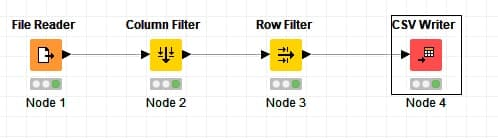
\includegraphics[width=0.9\linewidth]{figuras/capi 1/ejemplo_workflow}
	\caption{Ejemplo de flujo de trabajo en la herramienta KNIME.}
	\label{fig:ejemploworkflow}
\end{figure}

La herramienta KNIME puede ser extendida a través de plugins, la mayoría son nuevos nodos, aunque las extensiones pueden ser a cualquier parte de la arquitectura. La extensibilidad de la herramienta es de forma sencilla, ya que está basada en la Plataforma de Cliente Enriquecido de Eclipse (\textit{Eclipse RCP}, por sus siglas en inglés) \citep{berthold2009knime}. Gracias a esto, la adición de nuevos plugins a KNIME se torna menos compleja para el desarrollador. \\
KNIME se diseñó en base a tres principios: modularidad, extensibilidad y ambiente de trabajo interactivo. A continuación, se describen estos principios \citep{Lisandra2012}:

\begin{itemize}
	\item Modularidad: Plantea que no deben existir dependencias entre las unidades contenedoras de datos o de procesamiento. Además, se pueden implementar algoritmos de manera independiente. De igual forma, al no tener tipos de datos predefinidos, se pueden definir nuevos tipos de datos, con sus características y especificaciones propias. Estos pueden declararse compatibles con otros existentes.
	\item	Extensibilidad de forma sencilla: Permite adicionar nuevas unidades de procesamiento, visualización y tratamiento de datos, teniendo en cuenta que esto debe ser una tarea fácil de realizar.
	\item	Ambiente de trabajo visual e interactivo: Los flujos de trabajo deben ser fáciles e interactivos para el usuario. Por tal motivo, se harán arrastrando los elementos al área de trabajo.
\end{itemize}

Dado que se realiza la modificación de un componente en esta herramienta \citep{Carrazana2022}, se continuará el desarrollo en la misma.

\section{Componente KNIME de AutoML para el pre-procesado en tareas de clasificación}
AutoML en KNIME se refiere a la capacidad de la plataforma para automatizar el proceso de modelado de aprendizaje automático. Esto significa que los usuarios pueden cargar datos y permitir que la plataforma seleccione y optimice automáticamente el modelo que mejor se ajuste a los datos. Con tal objetivo, en \citep{Carrazana2022} se desarrolla un componente Componente KNIME de AutoML para el pre-procesado en tareas de clasificación. Este, a partir de un conjunto de datos y una columna objetivo, ejecuta diferentes flujos de pre-procesado, en aras de cumplir con los requisitos de los diferentes algoritmos de clasificación, siendo capaz de entrenarlos y probarlos, para posteriormente puntuar y graficar los resultados \citep{Carrazana2022}. En la figura \ref{fig:flujo-automl-componente} se muestra el flujo KNIME del componente AutoML Clasificación (pre-procesado).
\begin{figure}
	\centering
	\includegraphics[width=0.8\linewidth]{"figuras/capi 1/flujo-automl-componente"}
	\caption{Flujo KNIME del componente AutoML Clasificación (pre-procesado) \citep{Carrazana2022}}
	\label{fig:flujo-automl-componente}
\end{figure}
Este componente está enfocado en el pre-procesado de datos, donde se desarrollaron subcomponentes enfocados en la realización de las tareas de procesamiento de datos numéricos, string, valores faltantes, y el ajuste de tipos de columna. Como se observa en la figura \ref{fig:flujo-automl-componente}, se aplican los algoritmos de clasificación ID3, C4.5, CART, Redes Neuronales por retro propagación (RProp), Redes Neuronales Probabilísticas (PNN) y Máquina de Soporte Vectorial (SVM). Cada uno de estos requiere un tipo de pre-procesado diferente, acorde a los tipos de datos con los que trabaja. \\
\begin{figure}[H]
	\centering
	\includegraphics[width=0.4\linewidth]{"figuras/capi 1/pre-procesado-id3-ernesto"}
	\caption{Flujo de pre-procesado para el algoritmo ID3 \citep{Carrazana2022}}
	\label{fig:pre-procesado-id3-ernesto}
\end{figure}
No obstante hubo procesos que quedaron pendientes: la optimización de hiperparámetros y la automatización de algunas de las actividades esenciales en el pre-procesado, como la discretización y normalización de variables numéricas. Ambas pueden ser automatizadas acorde a la distribución que sigan los datos, sin embargo están configuradas de forma estática y no toman en cuenta lo anteriormente dicho. Por ejemplo, en la figura \ref{fig:pre-procesado-id3-ernesto} se muestra el nodo AutoBinner, empleado para la discretización, agrupando datos numéricos en intervalos (bins). De igual forma, la optimización de hiperparámetros no fue implementada en esta solución, siendo una de las tareas más importantes en AutoML para mejorar el rendimiento de los algoritmos empleados.

\section{Bases de datos de prueba}
Las bases de datos de prueba son conjuntos de datos creados para ayudar a los desarrolladores a probar y depurar aplicaciones de bases de datos sin tener que utilizar datos reales y confidenciales. Estas bases de datos de prueba contienen datos ficticios, pero siguen la estructura de una base de datos real, lo que permite a los desarrolladores probar la funcionalidad de la aplicación sin preocuparse por dañar datos importantes o comprometer la privacidad de los usuarios. \\
Kaggle Datasets y UCI Machine Learning Repository son dos de los repositorios en línea más populares para conjuntos de datos de prueba y de aprendizaje automático. \\
Kaggle Datasets es un sitio web de aprendizaje automático que ofrece una amplia variedad de conjuntos de datos de muestra, desde datos meteorológicos hasta datos de redes sociales. Los usuarios pueden buscar entre miles de conjuntos de datos y también pueden contribuir con sus propios conjuntos de datos. Kaggle también tiene una comunidad de científicos de datos y aprendizaje automático que pueden proporcionar comentarios y ayudar a los usuarios a mejorar sus modelos de aprendizaje automático. \\
Por otro lado, el UCI Machine Learning Repository es un repositorio de conjuntos de datos de muestra para aprendizaje automático, minería de datos y otras aplicaciones de análisis de datos. El repositorio fue creado por la Universidad de California, Irvine y contiene una amplia gama de conjuntos de datos, desde reconocimiento de voz hasta predicción de precios de viviendas. Los usuarios pueden descargar los conjuntos de datos de forma gratuita y utilizarlos para probar y desarrollar sus modelos de aprendizaje automático. \\
Ambos repositorios ofrecen una amplia variedad de conjuntos de datos, lo que los hace ideales para desarrolladores, estudiantes y profesionales de la ciencia de datos que buscan mejorar sus habilidades en el modelado de bases de datos y en la creación de modelos de aprendizaje automático precisos y efectivos. Por tal motivo, se emplearán ambos repositorios para la obtención de bases de datos para las pruebas que se realizarán más adelante.


\section{Conclusiones parciales}

% Cada conclusión tiene que estar sustentada en el cuerpo del capítulo.

A partir de lo estudiado en este capítulo, se llega a las siguientes conclusiones:

\begin{itemize}
	\item El Aprendizaje Automático es una técnica que permite a las computadoras aprender a partir de datos, sin necesidad de ser programadas explícitamente.
	\item El proceso de descubrimiento de conocimiento en bases de datos (KDD) es un proceso iterativo que consiste en varias etapas, incluyendo la selección de datos, la limpieza de datos, la transformación de datos y la minería de datos.
	\item La Minería de Datos es el proceso de descubrir patrones y relaciones interesantes en grandes conjuntos de datos, utilizando técnicas de aprendizaje automático, estadísticas y visualización de datos. Algunas de las técnicas utilizadas en la Minería de Datos incluyen la clasificación, la agrupación, la regresión y la asociación.
	\item La Clasificación es una técnica de aprendizaje automático que se utiliza para predecir la etiqueta o clase de un objeto a partir de un conjunto de características.
	\item El AutoML se puede utilizar para mejorar la eficiencia y la precisión del proceso de modelado, reducir la necesidad de conocimientos especializados y permitir a los usuarios enfocarse en la interpretación de los resultados. Las etapas del AutoML incluyen la selección automática de algoritmos, el preprocesamiento de datos, la optimización de hiperparámetros y la evaluación automática del modelo.
	\item El preprocesamiento de datos es una etapa crítica en el proceso de modelado, ya que los datos deben limpiarse, integrarse y transformarse antes de ser utilizados por los algoritmos de aprendizaje automático.
	\item Algunas de las tareas comunes del preprocesado de datos incluyen la eliminación de valores atípicos, el manejo de datos faltantes, la discretización y la normalización de datos numéricos.
	\item La discretización es una técnica utilizada para transformar datos numéricos en datos categóricos.
	\item Los hiperparámetros son ajustes que se realizan en los algoritmos de aprendizaje automático para mejorar su rendimiento. La optimización de hiperparámetros implica encontrar la combinación óptima de valores para los hiperparámetros.
	\item KNIME es una herramienta de minería de datos de código abierto que permite a los usuarios crear y ejecutar flujos de trabajo de análisis de datos.
\end{itemize}


%Una vez terminado el capítulo se arriban a las siguientes conclusiones:

%\begin{enumerate}
%	\setlength\itemsep{0em}
%	\item Una conclusión necesaria aquí son los requisitos principales que debe cumplir la solución propuesta.
%	\item Otra conclusión es la inexistencia de una solución que brinde cumplimiento a los requisitos planteados.
%	\item Finalmente, cuáles son las tecnologías seleccionadas y su justificación
%\end{enumerate}

\pagebreak
